\section{Introduction}

A Large Ion Collider Experiment (ALICE) has been proposed and built to study
the properties of the Quark-Gluon Plasma in hadronic collisions at the Large
Hadron Collider at CERN~\cite{Aamodt:2008zz}. The design was driven by the
requirement to cope with the high multiplicities in central \PbPb collisions
and provide a complete reconstruction of the events, including particle
identification over a wide \pt range.

The experimental setup consists of a central barrel contained in a solenoidal
magnet ($B = 0.5~\mathrm{Tesla}$) and a forward muon-system with a dipole magnet
providing $3~\mathrm{Tm}$, see Fig.~\ref{fig:alice_run2}. Until the end of Run~2,
the central barrel contained an Inner Tracking System (ITS) with two layers of
Silicon Pixel Detectors (SPD), two layers of Silicon Drift Detectors (SDD), and
two layers of Silicon Strip Detectors (SSD). In radial direction, it is followed
by a Time Projection Chamber (TPC) covering the radii from 0.5~m to 2.5~m over a
length of 7~m. \dots

\begin{itemize}
\item overview of the detector
  (status as of end of Run 2)
\item barrel tracking
\item detectors for particle identification
\item calorimetry
\item forward physics
\item triggering
\end{itemize}

\begin{figure}
\centering
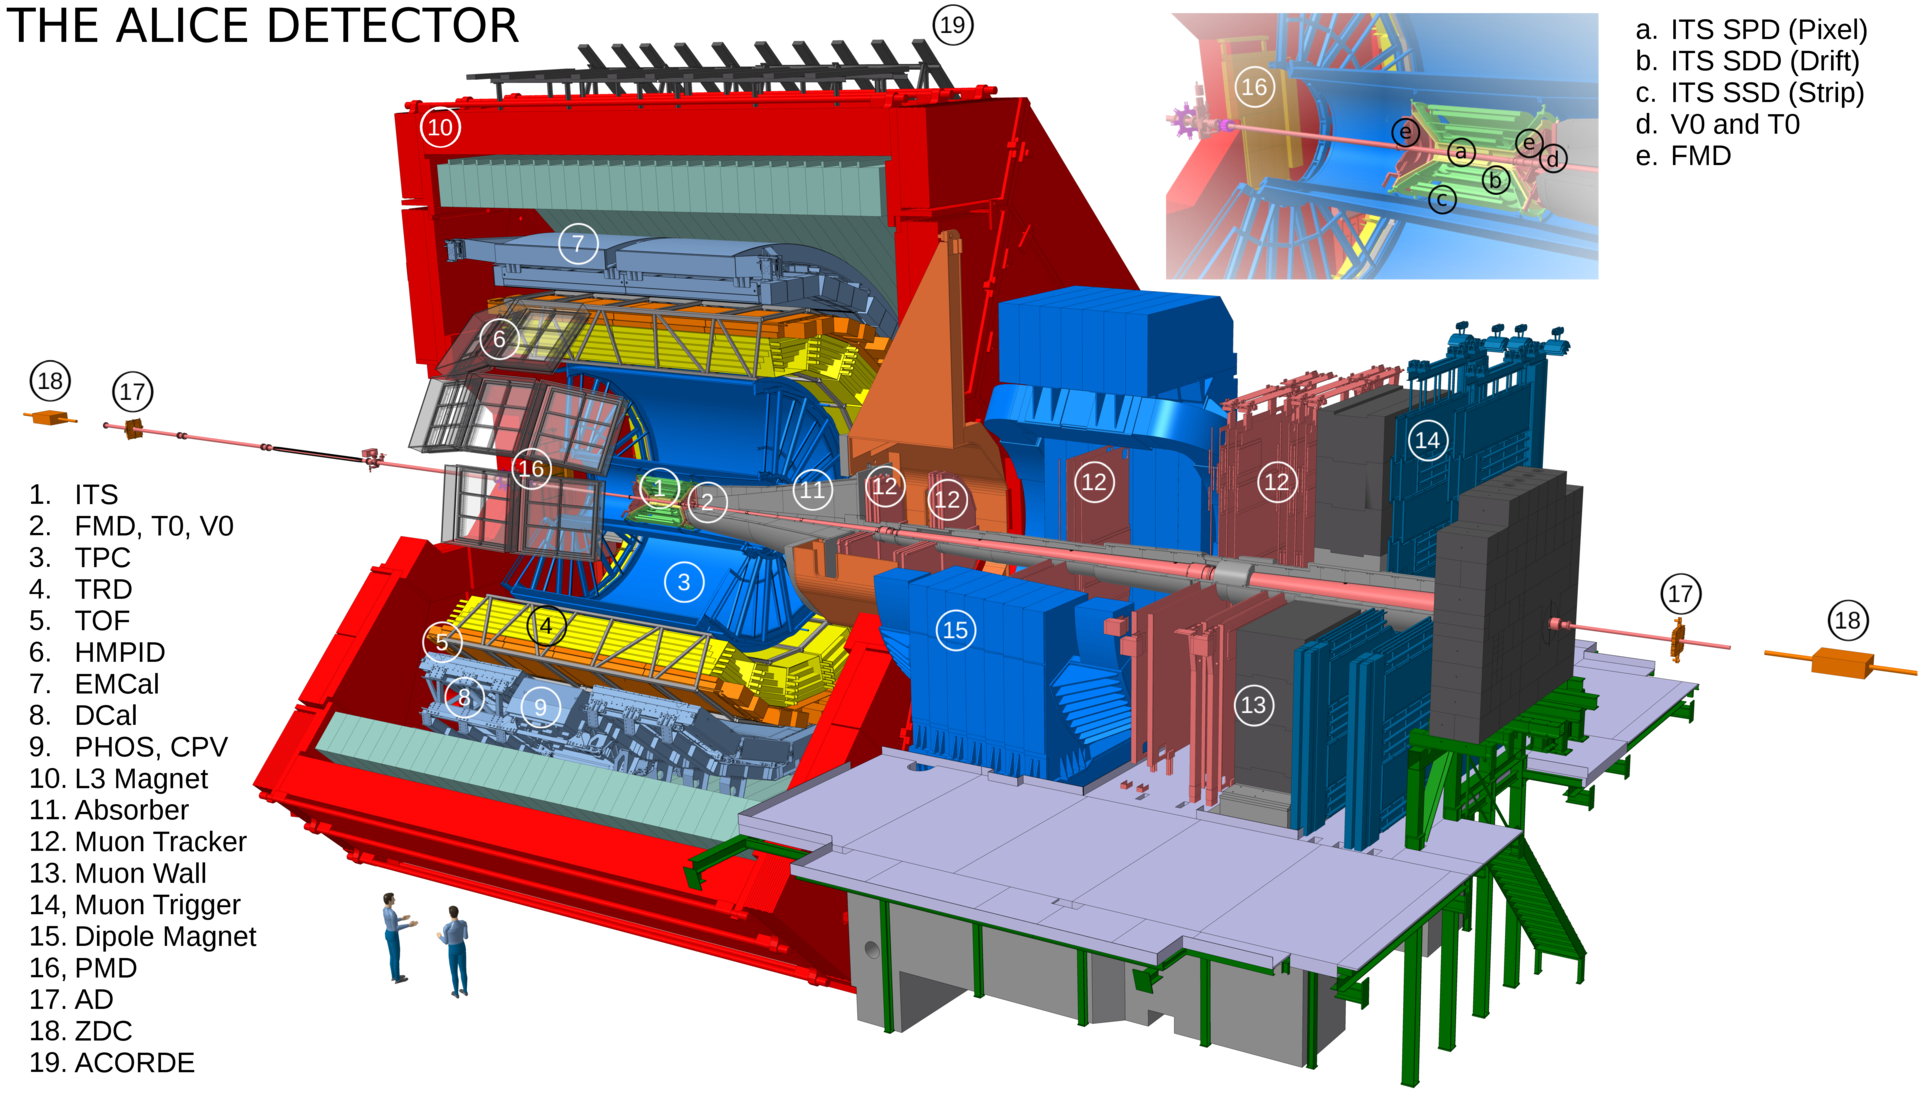
\includegraphics[width=.7\textwidth]{intro/2017-May-11-ALICE_RUN2_labels_HD}
\caption{Detector setup in Run 2}
\label{fig:alice_run2}
\end{figure}

\subsection{Run1/2 performance highlights (examples)}

cite performance paper~\cite{Abelev:2014ffa}, possibly also detector papers

discuss performance
\begin{itemize}
\item particle identification and relevant detectors
\item secondary vertex resolution
\item data sets (rate/integrated luminosity)
\end{itemize}

Data was recorded throughout the
running of the LHC in Run 1 and 2 exploiting a variety of collision systems and
energies, see Tab.~\ref{tab:datasets}.

\begin{table}
  \centering
  \rowcolors{2}{}{gray!30}
  \begin{tabular}{lrr}
    \multicolumn{1}{c}{system}
    & \multicolumn{1}{c}{$\snn~(\mathrm{\TeV})$}
    & \multicolumn{1}{c}{$L_\mathrm{int}$}\\
    \hline \hline
    \pp & 0.9 & $\sim 200~\mu\mathrm{b}^{-1}$\\
        & 2.76 & $\sim 100~\mathrm{nb}^{-1}$\\
        & 5.02 & $\sim 1.3~\mathrm{pb}^{-1}$\\
        & 7 & $\sim 1.5~\mathrm{pb}^{-1}$\\
        & 8 & $\sim 2.5~\mathrm{pb}^{-1}$\\
        & 13 & $\sim 25~\mathrm{pb}^{-1}$\\
    \pPb{} & 5.02 & $\sim 15 + 3~\mathrm{nb}^{-1}$\\
           & 8.16 & $\sim 25~\mathrm{nb}^{-1}$\\
    \XeXe{} & 5.44 & $\sim 0.3~\mu\mathrm{b}^{-1}$\\
    \PbPb{} & 2.76 & $\sim 75~\mu\mathrm{b}^{-1}$\\
            & 5.02 & $\sim 0.25 + 1~\mathrm{nb}^{-1}$\\
    \hline
  \end{tabular}
  \caption{ALICE datasets from LHC Run 1 and 2}
  \label{tab:datasets}
\end{table}
